\documentclass[journal=jpcbfk]{achemso}

\usepackage[version=3]{mhchem}
\usepackage[T1]{fontenc}
\newcommand*\mycommand[1]{\texttt{\emph{#1}}}
\newcommand{\todo}[1]{\textcolor{red}{#1}}

\usepackage{upgreek}				
\usepackage{xcolor}
\usepackage{booktabs}
\usepackage{multirow}
\usepackage{lmodern}
\usepackage{microtype}
\usepackage{xr}
\externaldocument{manuscriptPS}

\author{O. H. Samuli Ollila}
\email{samuli.ollila@helsinki.fi}
%\homepage[]{Your web page}
\affiliation{Institute of Organic Chemistry and Biochemistry,
Academy of Sciences of the Czech Republic, 
Prague 6, Czech Republic}
\affiliation{Institute of Biotechnology, University of Helsinki}

\author{NMRlipids collaboration \todo{Authorship query to be sent soon.}}
\affiliation{nmrlipids.blogspot.fi} 




\SectionNumbersOn

\renewcommand{\thetable}{S\arabic{table}}%
\renewcommand{\thefigure}{S\arabic{figure}}%
\renewcommand{\thesection}{S\arabic{section}}%
\renewcommand{\thepage}{S\arabic{page}}%

\title{ Supporting Information:\\ NMRlipids IV: Headgroup \& glycerol backbone structures, and cation binding in bilayers with PS lipids}

\begin{document}

\newpage
%\tableofcontents

\section{Simulated systems}

\subsection{CHARMM36}
\todo{To be written by Piggot, Madsen and Ollila}

\subsection{CHARMM36ua}
\todo{To be written by Piggot}

\subsection{Slipids}
\todo{To be written by Piggot and Favela}

\subsection{Berger}
\todo{To be written by Piggot and Ollila}
Simulations with excess sodium were taken directly from Ref. \citenum{jurkiewicz12} and
simulations with calcium directly from \citenum{melcrova16}.
Simulation of POPC at 310 K was taken directly from Ref. \citenum{ollila07a}.

\subsection{GROMOS-CKP}
\todo{To be written by Piggot}

\subsection{Lipid17}
\todo{To be written by Kav, Miettinen and Meclr.}

\subsection{MacRog}
\todo{To be written by Javanainen and Piggot}


\section{Electrometer concept in PC lipid bilayers mixed with negatively charged lipids}\label{electrometerFORmixtures}

The electrometer concept is based on the empirical observations that
the order parameters of $\alpha$ and $\beta$ carbons in PC lipid headgroup
decrease (increase) proportionally to the bound positive (negative) 
charge~\cite{akutsu81,altenbach84,seelig87,scherer89}. 
The concept is also valid for lipid mixtures where PC order parameters 
increase when mixed with anionic lipids, in contrast to the mixtures with neutral or
cationic surfactants~\cite{seelig87, scherer87} (Fig. \ref{HGorderparametersPCvsPEPSPGchol}).
\begin{figure}[]
  \centering
  \includegraphics[width=8.0cm]{../Figs/HGorderparametersPCvsPEPSPGchol.eps}
  \caption{\label{HGorderparametersPCvsPEPSPGchol}
    PC headgroup order parameters from experiments of mixtures with
    PE, PS, PG and cholesterol \cite{scherer87,scherer89,ferreira13}.
    Signs are determined as discussed in \cite{botan15,ollila16}.
  }
\end{figure}

Based on the electrometer concept, the headgroup order parameters of
PC lipids can be used to measure the ion binding affinity to lipid 
bilayers \cite{akutsu81,altenbach84,seelig87}. Changes of the headgroup order 
parameters of negatively charged PS and PG lipids with bound charge are also systematic,
but less well characterized~\cite{borle85,macdonald87,roux86,roux90}.
Therefore, the ion binding affinity to negatively charged bilayers
can be better characterized measuring the PC headgroup order parameters from 
mixed bilayers. The PC headgroup order parameters in mixtures with anionic
lipids are larger than in pure PC lipid because addition of
negative charges increase the order parameters (Figs. \ref{HGorderparametersPCvsPEPSPGchol} 
and \ref{OrderParametersWithCaCl}). Upon addition of CaCl$_2$, the PC headgroup order 
parameters in the mixed bilayers decrease and reach the values of pure PC bilayer close 
to the CaCl$_2$ concentrations of $\sim$ 50-300mM, depending on the amount of negatively charged
lipids in the mixture (Fig. \ref{OrderParametersWithCaCl}). At this point the charge of
bound Ca$^{2+}$ probably cancels the charge of anionic negative lipids and the bilayer 
has neutral charge. The overcharging then occurs with larger concenterations.
\begin{figure}[]
  \centering
  \includegraphics[width=8.0cm]{../Figs/LIPIDSwithCaCl.eps}
  \includegraphics[width=8.0cm]{../Figs/LIPIDSwithCaClBELOW1M.eps}
  \caption{\label{OrderParametersWithCaCl}
    PC headgroup order parameters as a function of CaCl concentration from experiments 
    different mole fractions of negatively charged lipids.
    Pure DPPC data from \cite{akutsu81}, pure POPC data from \cite{altenbach84}, 
    POPC:POPS mixture data from \cite{roux90}, POPC:POPG mixture data with 0.1M NaCl from \cite{macdonald87}
    and POPC:POPG mixture data without NaCl from \cite{borle85}.
    The right column shows the results zoomed to concentrations below 1M.
  }
\end{figure}
As expected, the more pronounced order parameter decrease is observed in systems with more
negatively charged lipids (Fig. \ref{OrderParameterCHANGESWithCaClBELOW1M}) indicating 
higher binding affitiny of cations into the negatively charged membranes. In conclusion,
the consistency of the experimental results suggests that the electrometer concept can
be used to determine the cation binding also to the lipid bilayers containing negatively
charged lipids.  
\begin{figure}[]
  \centering
  \includegraphics[width=9.0cm]{../Figs/CHANGESwithCaCl.eps}
  \caption{\label{OrderParameterCHANGESWithCaClBELOW1M}
    The change of PC headgroup order parameters as a function of CaCl$_2$
    measured from bilayers containing different amount of negatively charged lipids.
    The values are taken from 2H NMR experiments reported in the
    literature (DPPC \cite{akutsu81}, POPC \cite{altenbach84}, POPC:POPS (5:1) \cite{roux90},
    POPC:POPG  mixtures with 0.1M NaCl \cite{macdonald87}
    and POPC:POPG (1:1) without NaCl \cite{borle85}).
    As expected, the decrease of order parameters with the added CaCl$_2$
    is more pronounced for systems with larger fraction of
    negatively charged lipids, indicating larger amount amount
    of bound cations.
  }
\end{figure}

\pagebreak
\section{Calibration of PC headgroup order parameter response to the bound cations}\label{electrometerCALIBRATION}
Before using the headgroup order parameters to compare ion binding affinity between simulations
and experiments, it is important to quantify the response of the order parameters to the
bound charge in simulations~\cite{catte16,melcr18}. Comparison of the headgroup order parameter
response to the cationic surfactants in POPC bilayer to the experiments \cite{scherer89} shows
that the both order parameters are too sensitive to the bound charge in the Lipid14 model,
while CHARMM36 gives better agreement for the $\alpha$ carbon (Fig. \ref{CHANGESwithDHMDMAB}).
The ratio $\Delta S_{\rm CH}^\beta / \Delta S_{\rm CH}^\alpha$ from Lipid14 model was in good agreement 
with experiments in the previous study~\cite{catte16} because both order parameters are equally too 
sensitive to the bound cations (Fig. \ref{CHANGESwithDHMDMAB}). The ratio was, however, overestimated
for the CHARMM36 model because the $\beta$ order parameter relatively more sensitive than the $\alpha$
order parameter. These have to be taken into account when analysing the ion binding affinities
using headgroup order parameters in simulations.
\begin{figure}[]
  \centering
  \includegraphics[width=9.0cm]{../Figs/HGopsDHMDMAB.eps}
  \caption{\label{CHANGESwithDHMDMAB}
  The response of headgroup order parameters to the fixed amount of cationic surfactants in
  POPC bilayer is compared between simulations and experiments \cite{scherer89}.}
\end{figure}

\pagebreak
\section{Difference between POPC and OPPS in MacRog model}

\begin{figure}[]
  \centering
  \includegraphics[width=9.0cm]{../Figs/HGorderparametersPOPSvsOPPS.eps}
  \caption{\label{CHANGESwithCaClPGPS}
    Headgroup order parameters from POPS and OPPS simulations with MacRog model.}
\end{figure}

\pagebreak
\section{Dihedrals}
\begin{figure*}[]
  \centering
  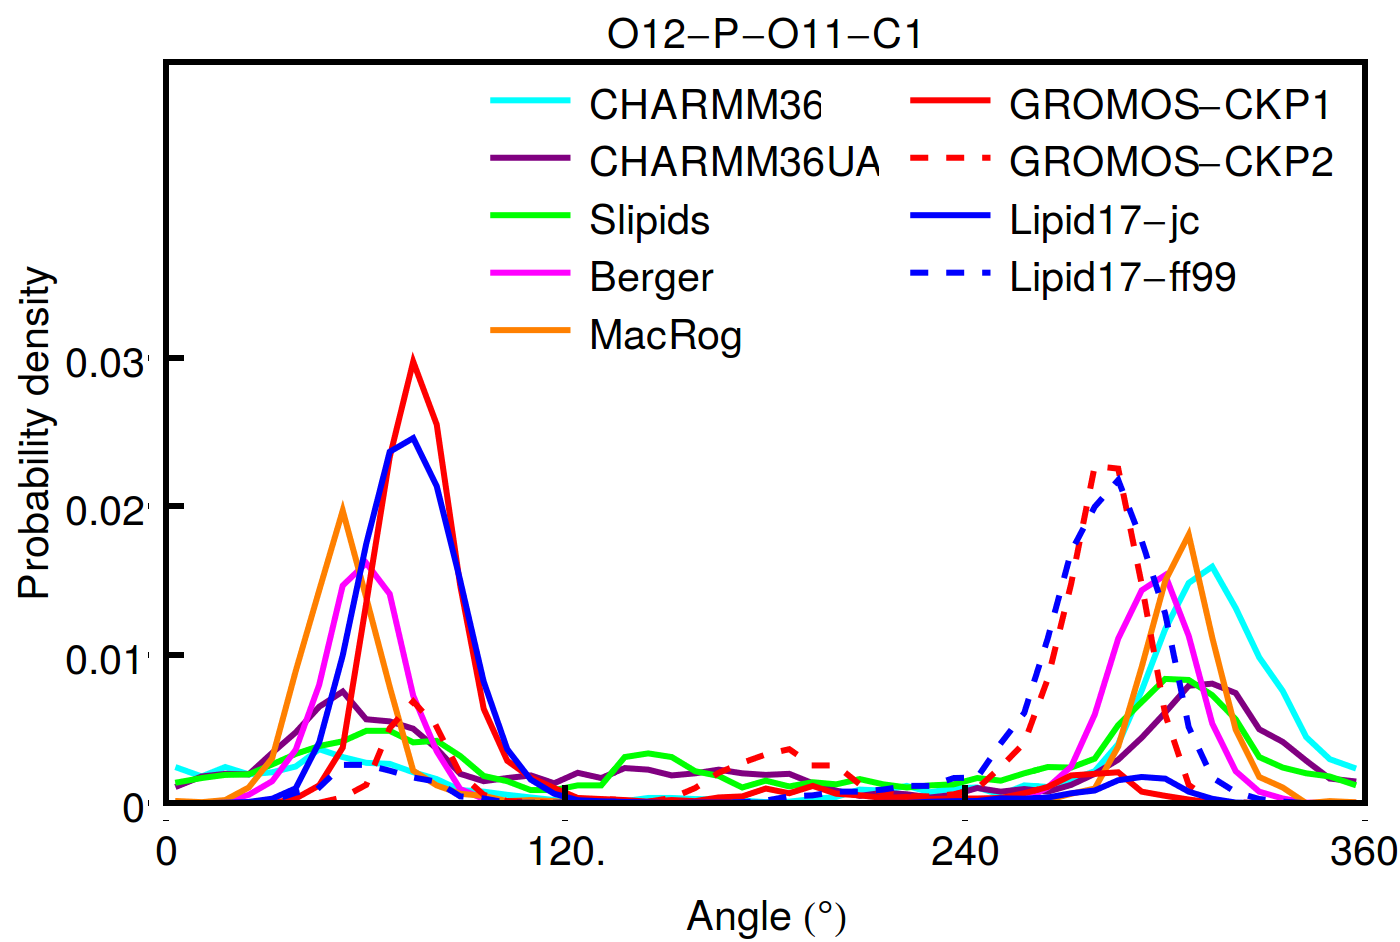
\includegraphics[width=8.0cm]{../Figs/diheds_pops1.png}
  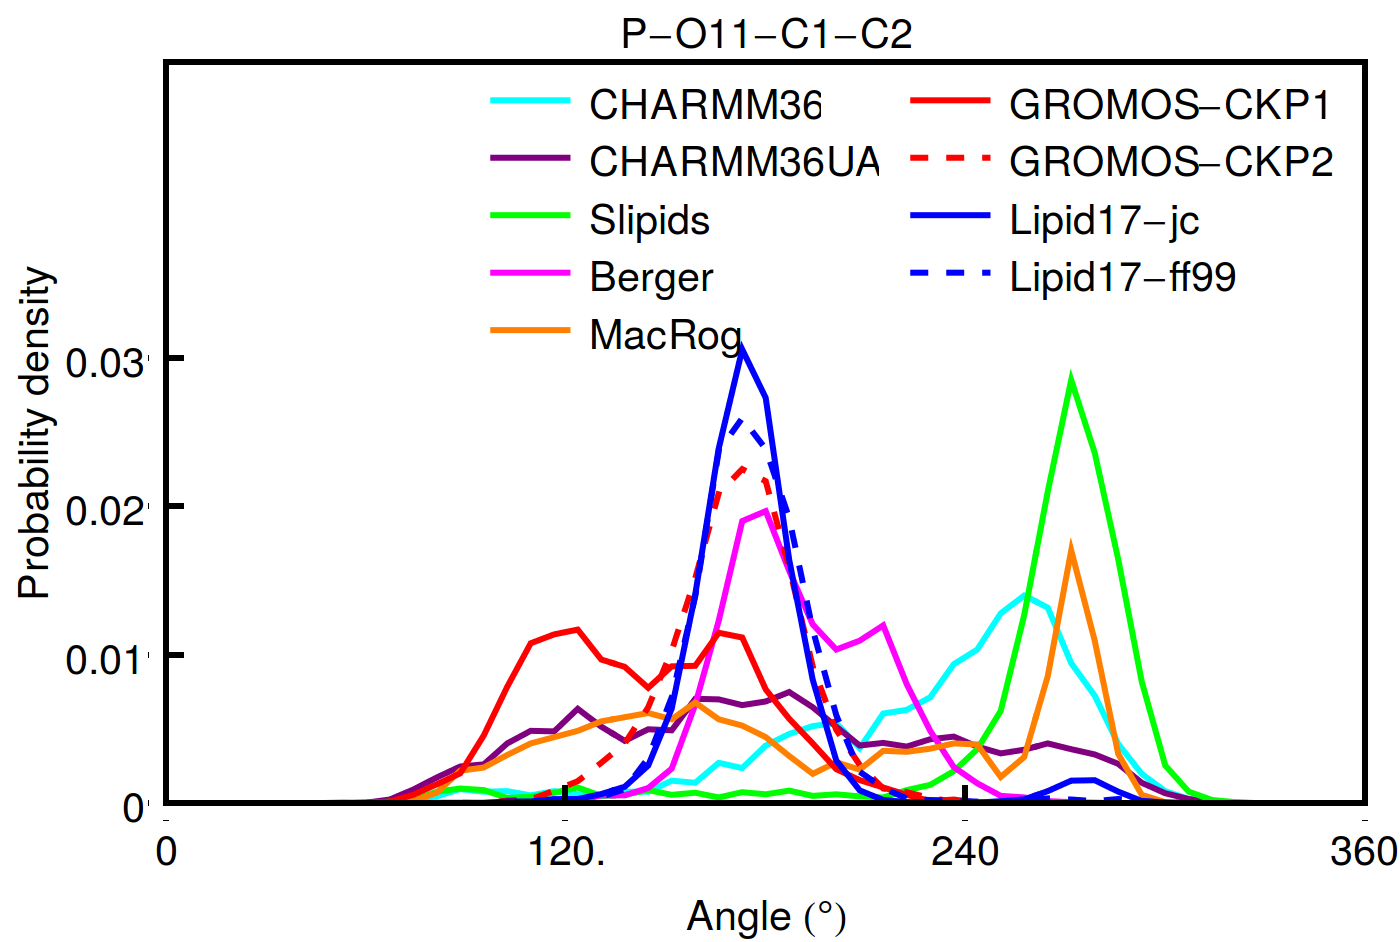
\includegraphics[width=8.0cm]{../Figs/diheds_pops2.png}
  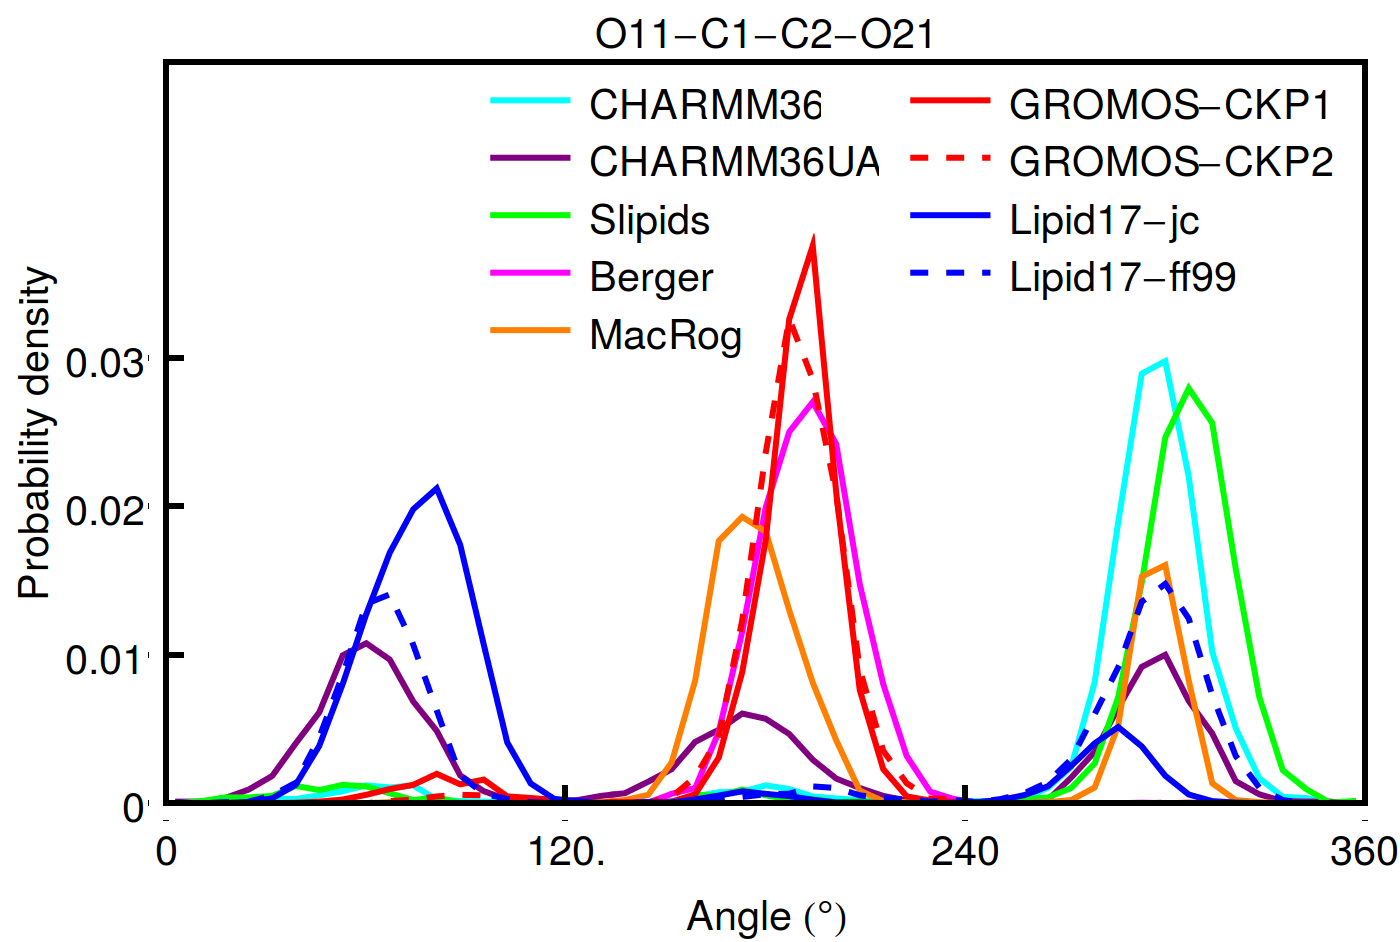
\includegraphics[width=8.0cm]{../Figs/diheds_pops3.png}
  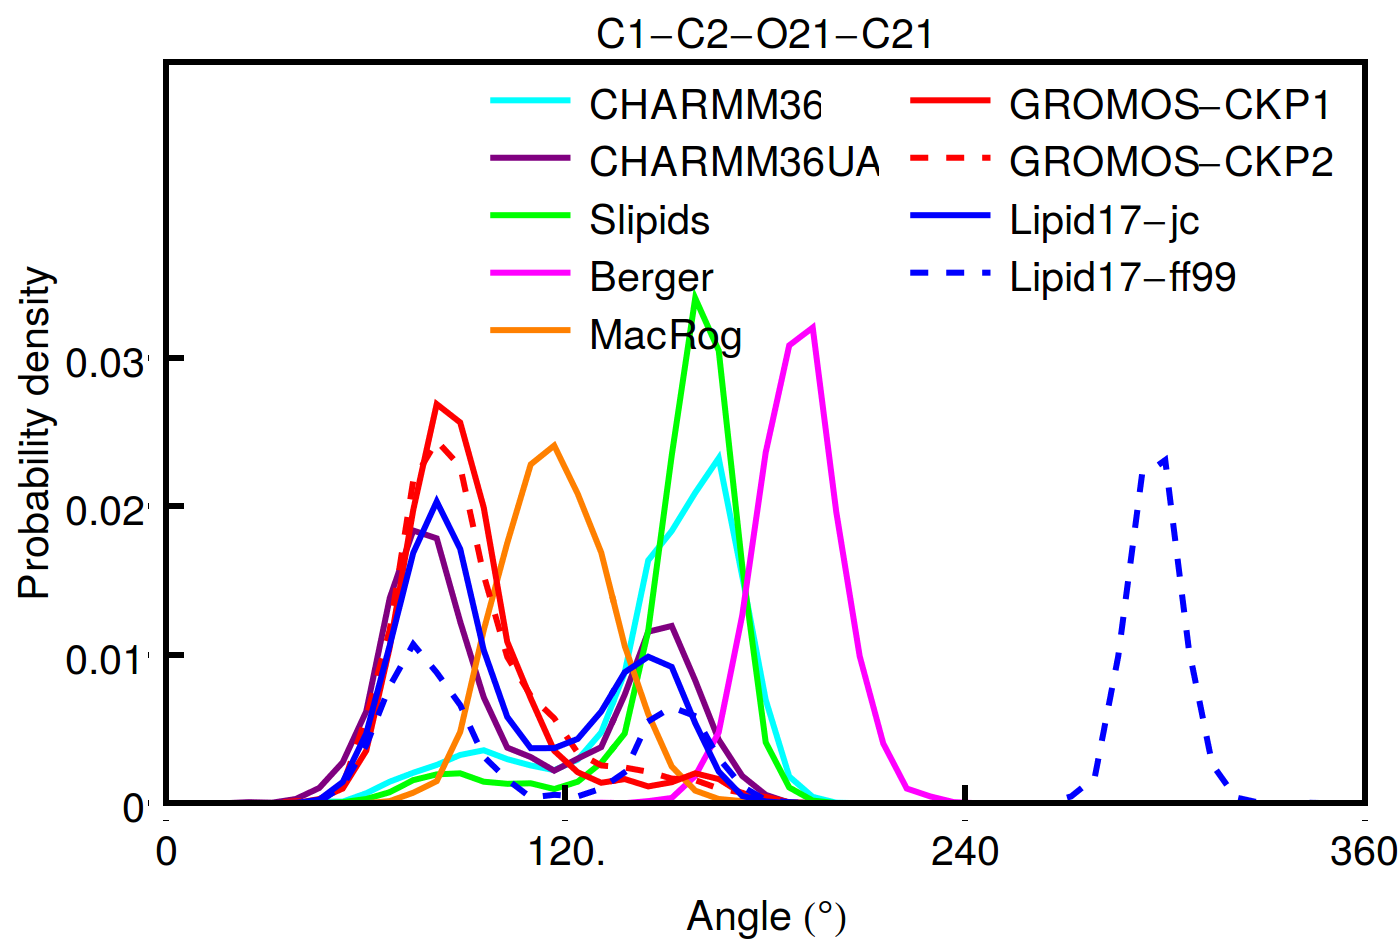
\includegraphics[width=8.0cm]{../Figs/diheds_pops4.png}
  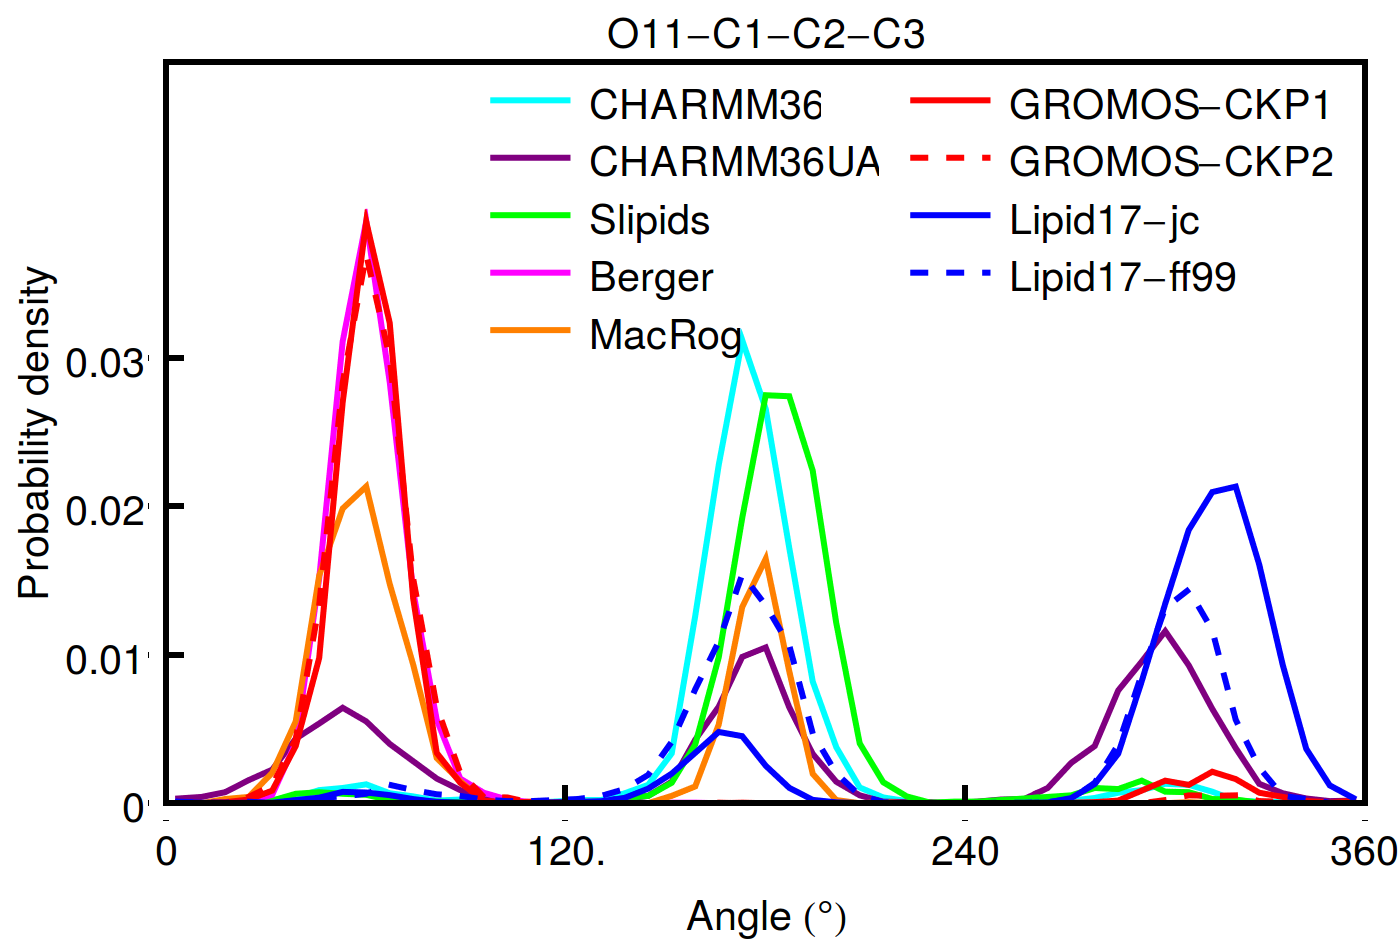
\includegraphics[width=8.0cm]{../Figs/diheds_pops5.png}
  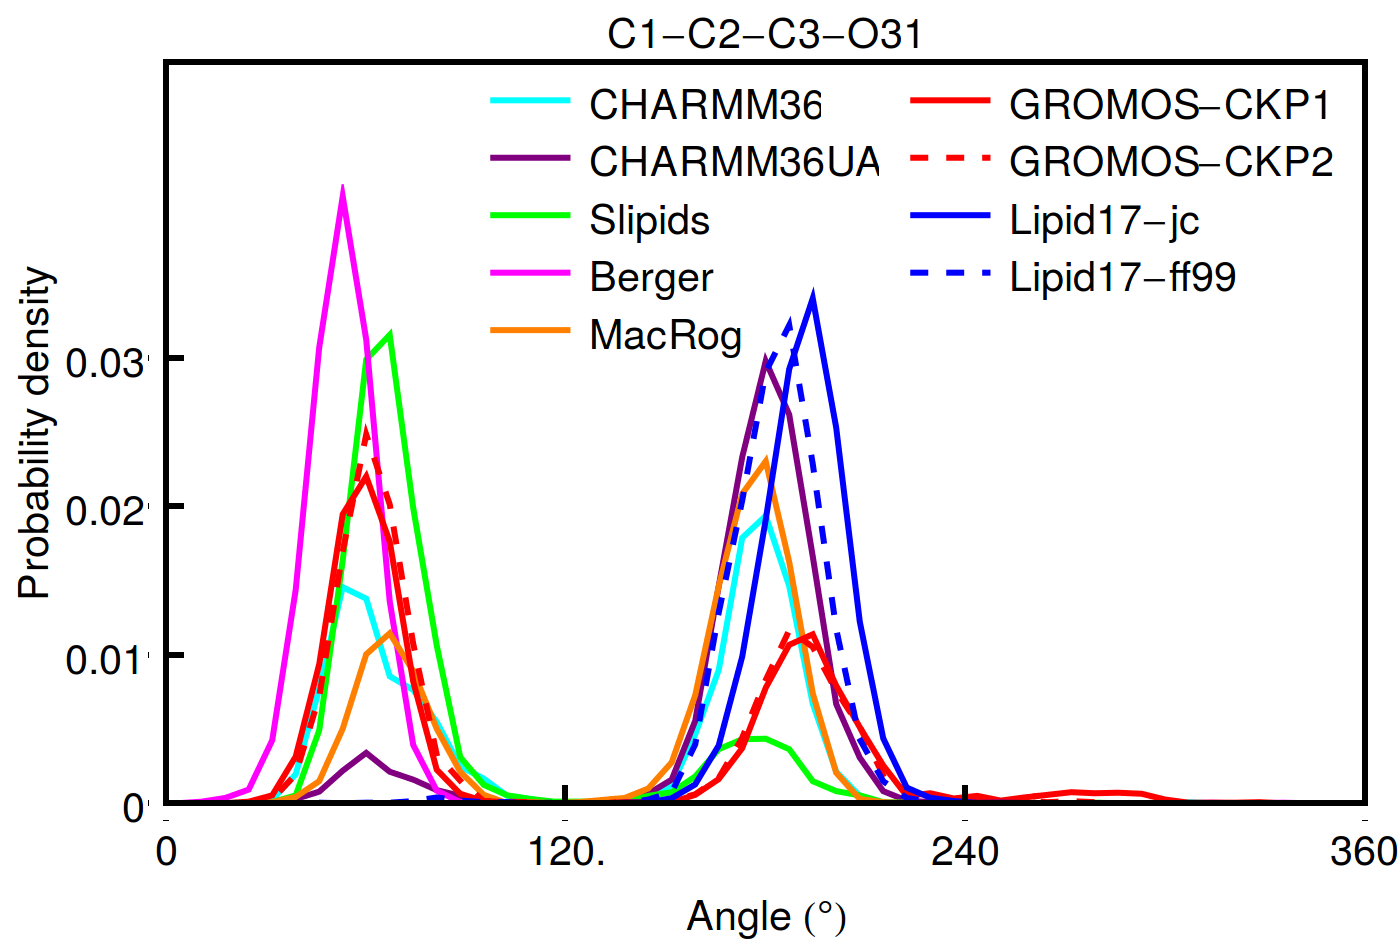
\includegraphics[width=8.0cm]{../Figs/diheds_pops6.png}
  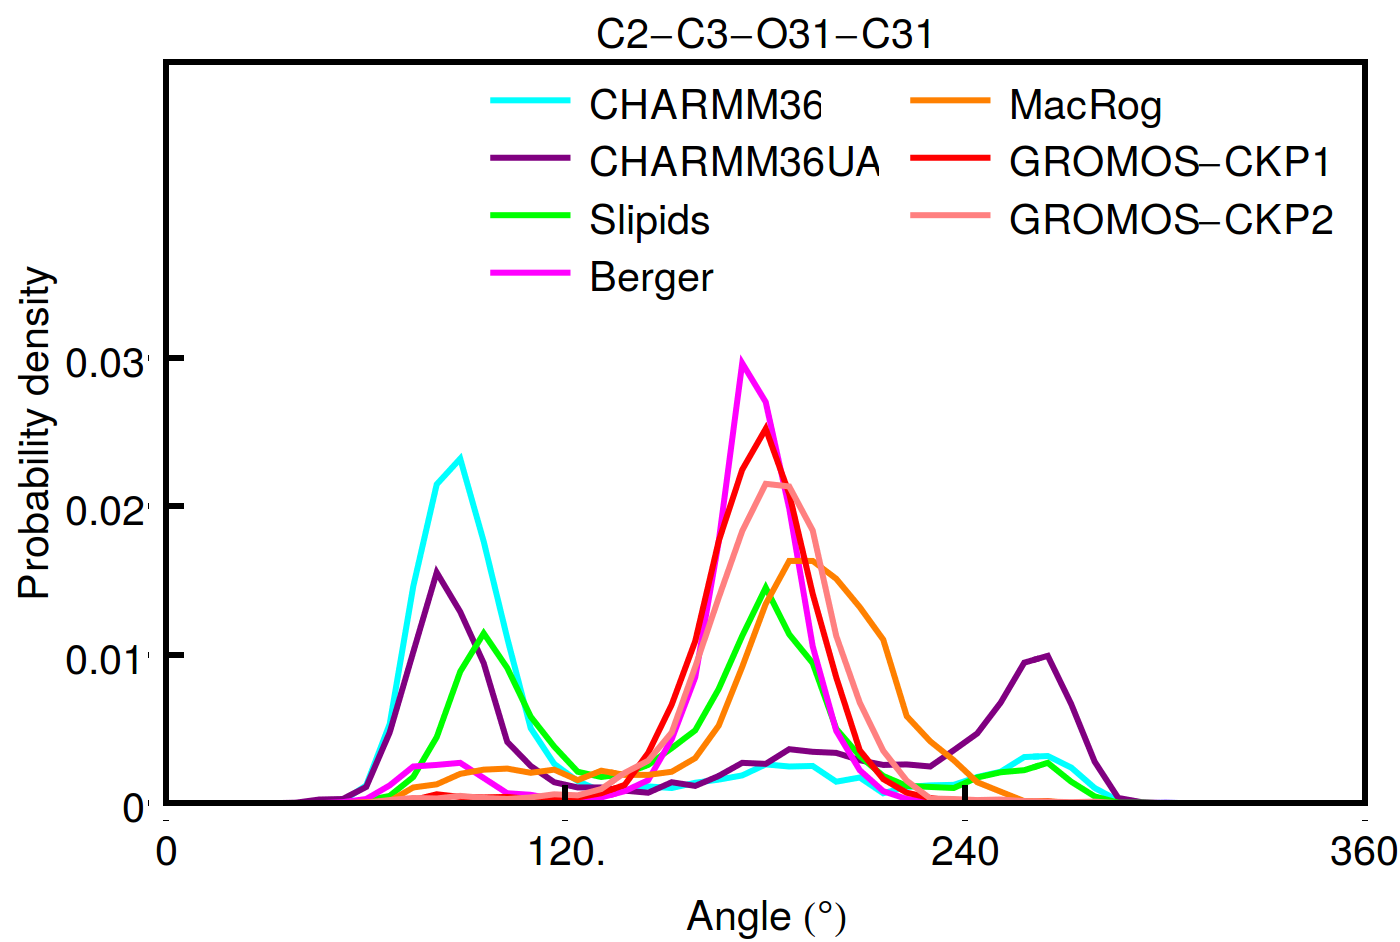
\includegraphics[width=8.0cm]{../Figs/diheds_pops7.png}
  \caption{\label{dihedralsGLY}
    Dihedral angle distributions of bonds from phosphate to acyl chain carbonyls from different simulation models.
  }
\end{figure*}

\begin{figure*}[]
  \centering
  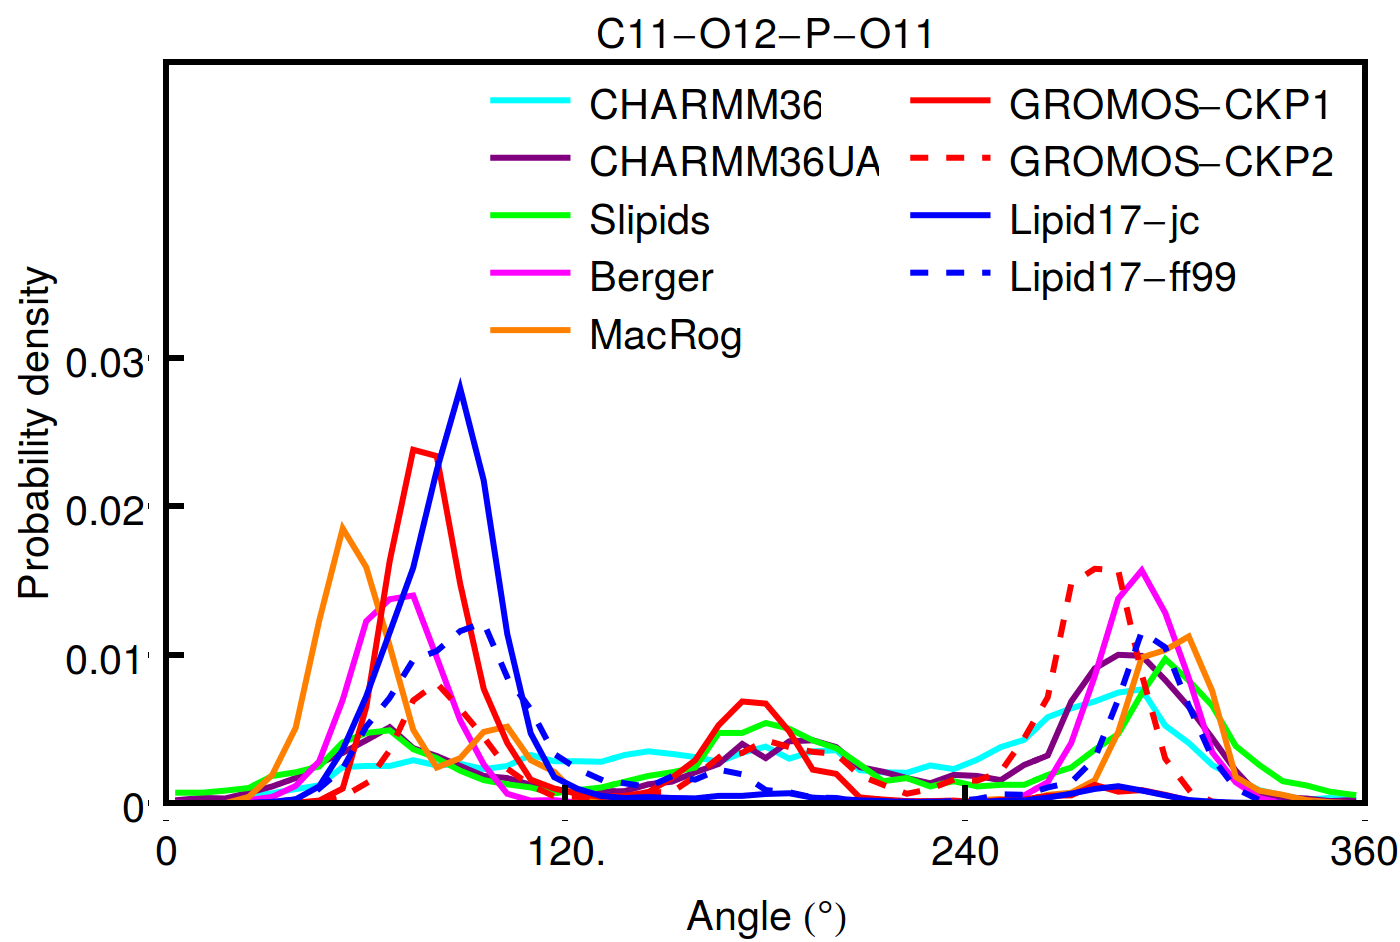
\includegraphics[width=8.0cm]{../Figs/diheds_pops8.png}
  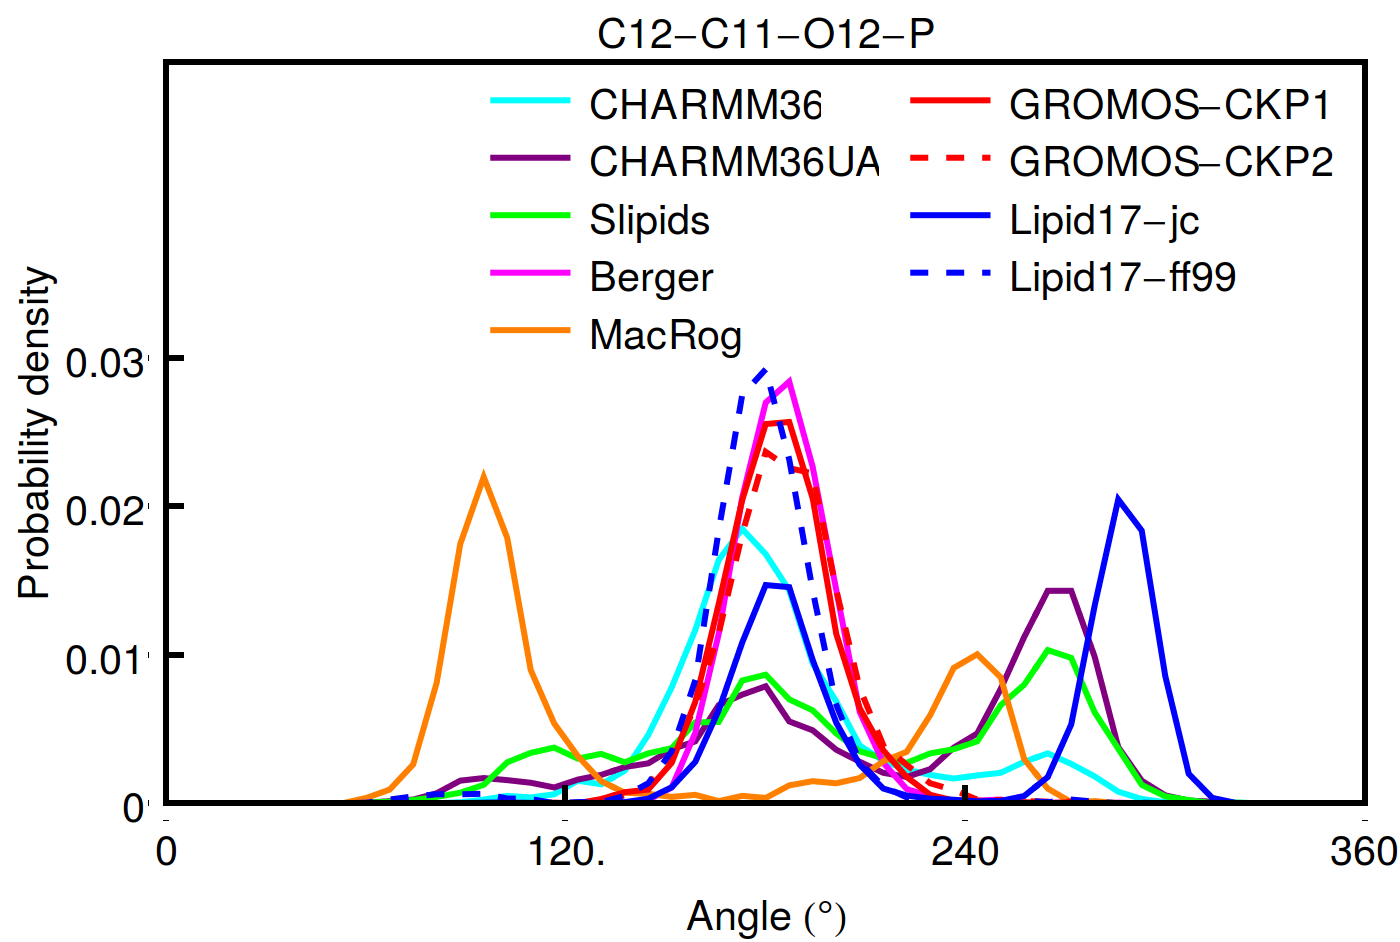
\includegraphics[width=8.0cm]{../Figs/diheds_pops9.png}
  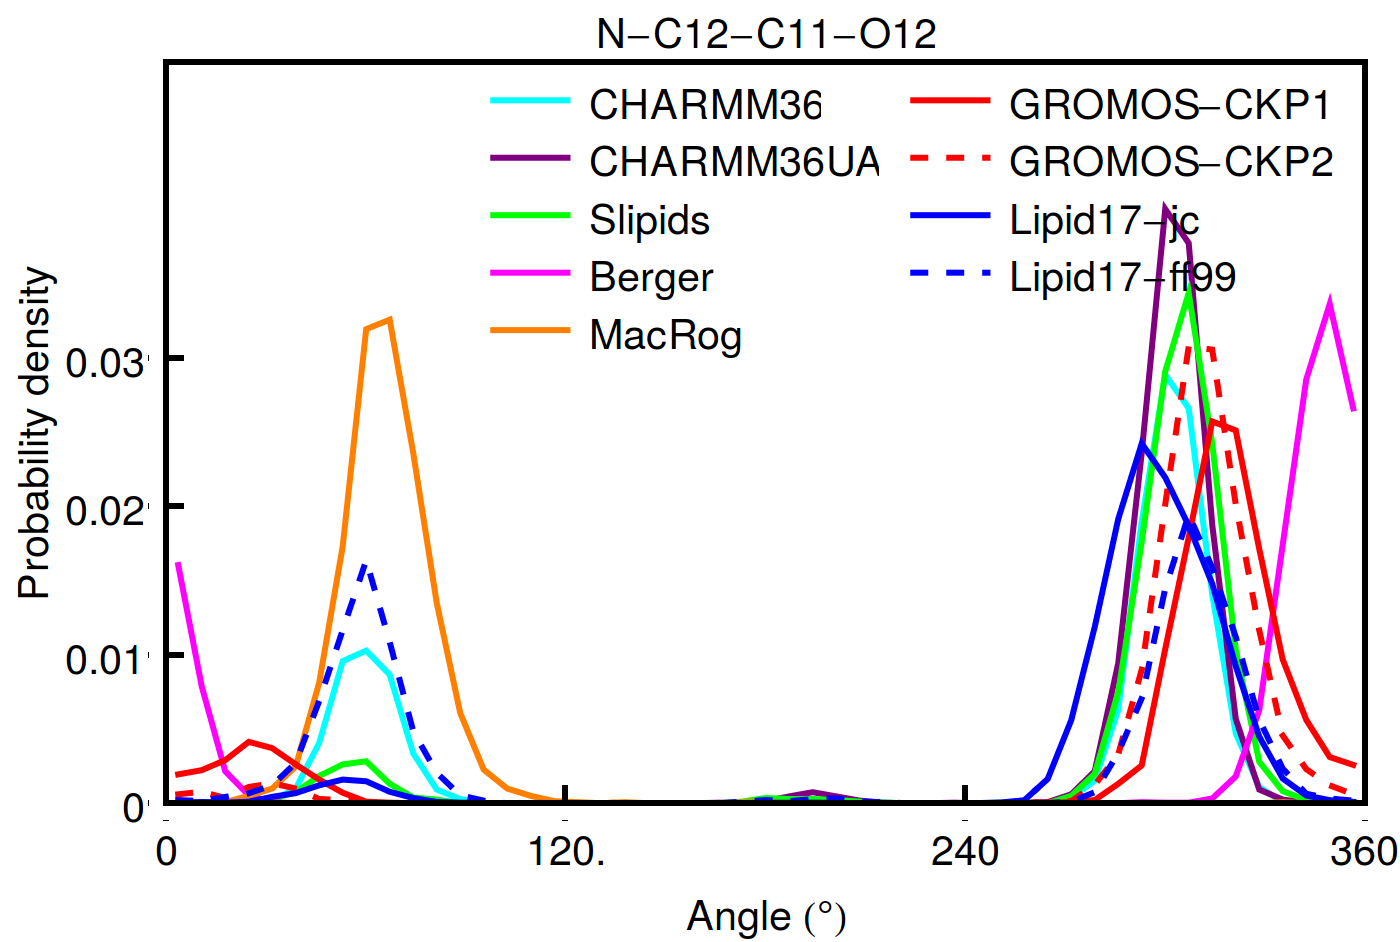
\includegraphics[width=8.0cm]{../Figs/diheds_pops10.png}
  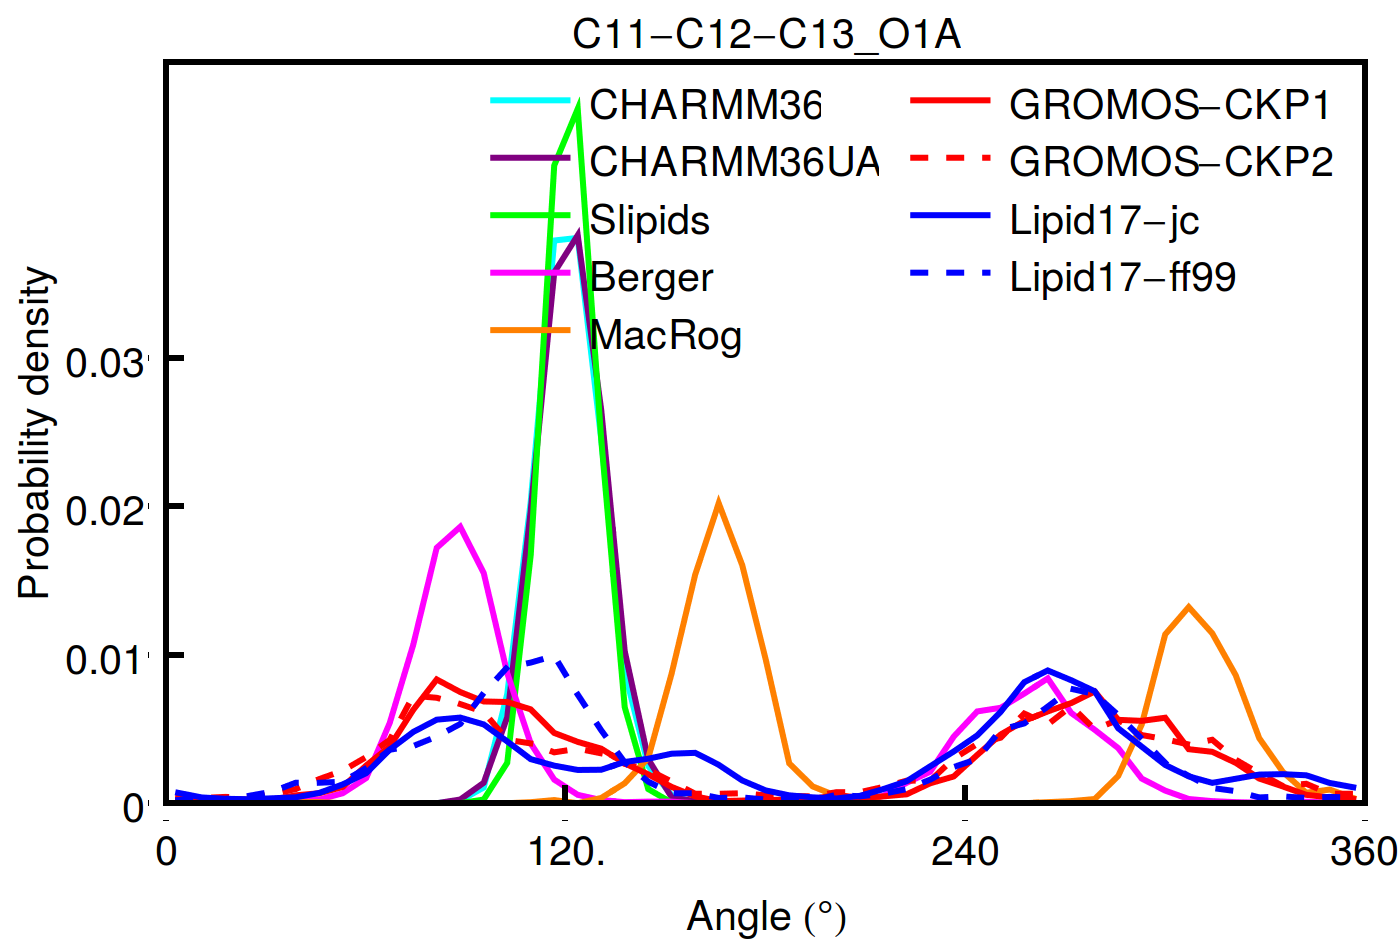
\includegraphics[width=8.0cm]{../Figs/diheds_pops11.png}
  \caption{\label{dihedralsHG}
    Dihedral angle distributions of bonds from phosphate to headgroup from different simulation models.
  }
\end{figure*}

\begin{figure}[]
  \centering
  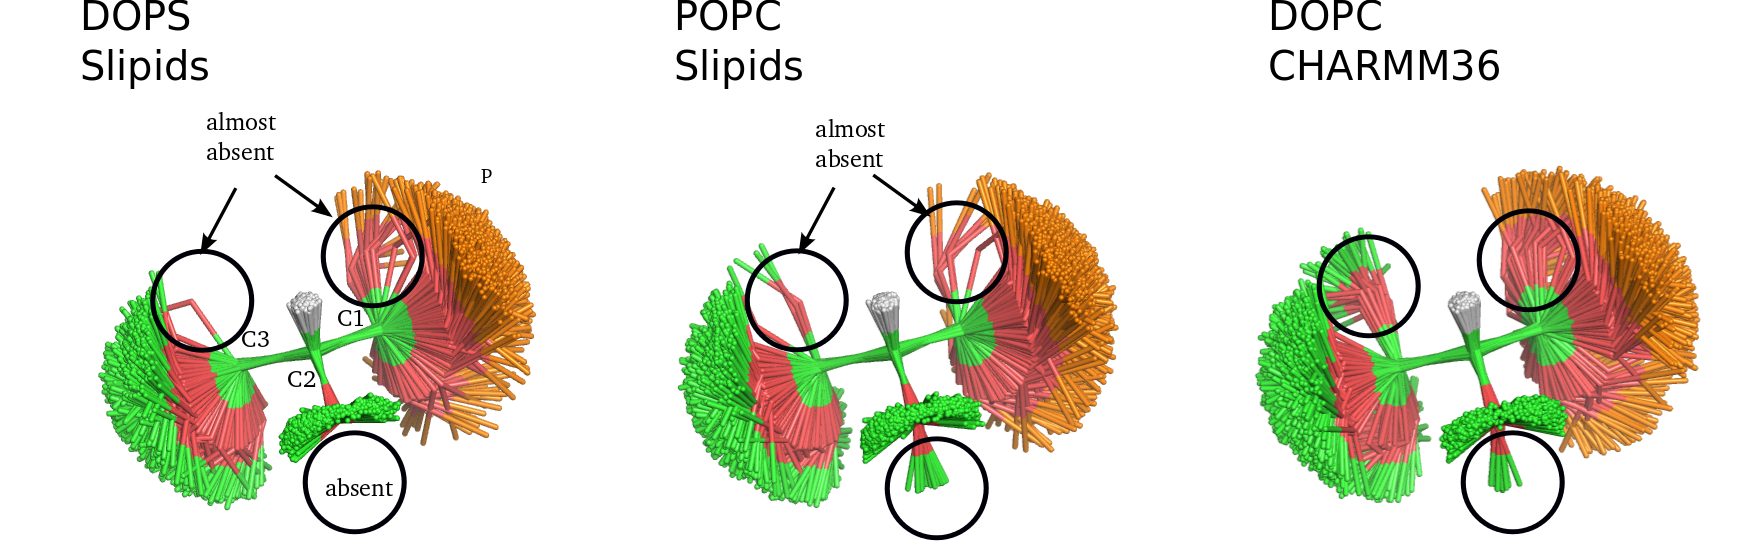
\includegraphics[width=9.0cm]{../Figs/glycerol_buslaev.png}
  \caption{\label{glycerol_buslaev}
    Snapshots overlayed from different simulations for glycerol backbone region
    by Pavel Buslaev.
  }
\end{figure}
\pagebreak

\section{Sodium binding to DMPC:DOPS mixture}

\begin{figure}[]
  \centering
  \includegraphics[width=9.0cm]{../Figs/PSresponseTONaCl.eps}
  \caption{\label{PSresponseTONaClDMPC}
    Order parameters of PS headgroup as a function of added NaCl measured from DMPC:DMPS (3:1) mixture \cite{roux86}.
  }
\end{figure}
The experimental results show essentially no changes in the order parameters as a function of
added NaCl, while significant changes are observed in simulations. However,
the minimum buffer concentration of NaCl in the experimental was 100mM \cite{roux86}.
Therefore, we cannot exclude the possibility that the NaCl induced changes were already
saturated with 100mM NaCl concentration, which was the case for CaCl$_2$ in Fig. \ref{changesWITHCaClPS}.
\pagebreak

\section{Calcium bindinf to POPC in CHARMM36 simulation with NBfix}

\begin{figure}[]
  \centering
  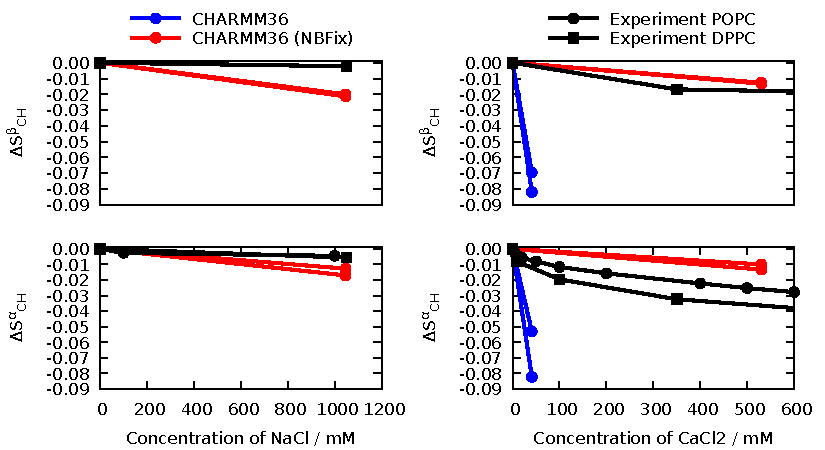
\includegraphics[width=9.0cm]{../Figs/OP_CHARMM_CaCl_POPC_NBFix.pdf}
  \caption{\label{OP_CHARMM_CaCl_POPC_NBFix}
  The response of headgroup order parameters to the fixed amount of cationic surfactants in
  POPC bilayer is compared between simulations and experiments \cite{scherer89}.}
\end{figure}

\begin{figure}[]
  \centering
  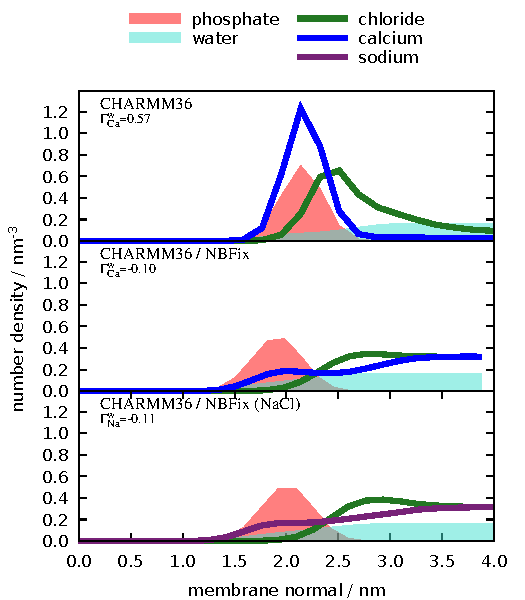
\includegraphics[width=9.0cm]{../Figs/density_profile_CHARMM_CaCl_POPC_NBFix.pdf}
  \caption{\label{density_profile_CHARMM_CaCl_POPC_NBFix}
  The response of headgroup order parameters to the fixed amount of cationic surfactants in
  POPC bilayer is compared between simulations and experiments \cite{scherer89}.}
\end{figure}

\pagebreak
\section{Details of the rough subjective force field ranking (Fig.~\ref{comparisonTablePS})} 

The assessment was based fully on the Fig.~\ref{HGorderParametersPS}.
%
First, for each carbon (the columns in Fig.~\ref{HGorderParametersPS}) in each force field (the rows),
we looked separately at deviations in magnitude and forking.

{\bf Magnitude} deviations, i.e., how close to the experimentally obtained C--H order parameters (OPs)
the force-field-produced OPs were.
%
For each carbon, the following 5-step scale was used:
%
\begin{description}
\item [0 (~):] \noindent {More than half of all the calculated OPs (that is, of all different hydrogens in all different lipids) were within the {\it subjective sweet spots} (SSP, blue-shaded areas in Fig.~\ref{HGorderParametersPS}).}
%
\item [1 ({\textsf{\tiny M}}):] \noindent {All the calculated OPs  were $< 0.03$ units away from the SSP.}
%
\item [2  ({\textsf{\small M}}):] \noindent {All the calculated OPs  were $< 0.05$ units away from the SSP.}
%
\item [3 ({\textsf{\large M}}):] \noindent {All the calculated OPs  were $< 0.10$ units away from the SSP.}
%
\item [4 ({\textsf{\Large M}}):] \noindent {Some of the calculated OPs  were $> 0.10$ units  away from the SSP.}
\end{description}

{\bf Forking} deviations, i.e., how well the difference in order parameters of two hydrogens attached to a given carbon matched that obtained experimentally. Note that this is not relevant for $\beta$ and $\mathrm{g_2}$, which have only one hydrogen. For the $\alpha$ carbon,  for which a considerable forking of 0.105 is experimentally seen, the following 5-step scale was used:
\begin{description}
\item [0 (~):] \noindent {The distance $D$ between the dots (that mark the measurement-time-weighted averages in Fig.~\ref{HGorderParametersPS}) was $0.08 < D< 0.13$ units for all the calculated OPs (that is, for all different lipids).}
%
\item [1 ({\textsf{\tiny F}}):] \noindent {$(0.06 < D < 0.08)$ OR $(0.13 < D < 0.15)$.}
%
\item [2  ({\textsf{\small F}}):] \noindent {$(0.04 < D < 0.06)$ OR $(0.15 < D < 0.17)$.}
%
\item [3 ({\textsf{\large F}}):] \noindent {$(0.02 < D < 0.04)$ OR $(0.17 < D < 0.19)$.}
%
\item [4 ({\textsf{\Large F}}):] \noindent {$(D<0.02)$ OR $(0.19<D)$.}
\end{description}
%
For the $\mathrm{g_3}$ carbon, for which no forking is indicated by experiments, the following 5-step scale was used:
%
\begin{description}
\item [0 (~):] \noindent {$ D< 0.02$.}
%
\item [1 ({\textsf{\tiny F}}):] \noindent {$0.02 < D < 0.04$.}
%
\item [2  ({\textsf{\small F}}):] \noindent {$0.04 < D < 0.06$.}
%
\item [3 ({\textsf{\large F}}):] \noindent {$0.06 < D < 0.08$.}
%
\item [4 ({\textsf{\Large F}}):] \noindent {$0.08 < D$.}
\end{description}
%
For the $\mathrm{g_1}$ carbon, for which a considerable forking of 0.13 is experimentally seen, the following 5-step scale was used:
%
\begin{description}
\item [0 (~):] \noindent {$0.11 < D < 0.15$.}
%
\item [1 ({\textsf{\tiny F}}):] \noindent {$(0.09 < D < 0.11)$ OR $(0.15 < D < 0.17)$.}
%
\item [2  ({\textsf{\small F}}):] \noindent {$(0.07 < D < 0.09)$ OR $(0.17 < D < 0.19)$.}
%
\item [3 ({\textsf{\large F}}):] \noindent {$(0.05 < D < 0.07)$ OR $(0.19 < D < 0.21)$.}
%
\item [4 ({\textsf{\Large F}}):] \noindent {$(D<0.05)$ OR $(0.21<D)$.}
\end{description}

Based on these assessments of magnitude and forking deviations,
each carbon was then assigned to one of the following groups:
"within experimental error"
(magnitude and forking deviations both on step 0 of the scales described above),
"almost within experimental error"
(sum of the magnitude and forking deviation steps 1 or 2),
"clear deviation from experiments"
(sum of magnitude and forking deviation steps from 3 to 5), and
"major deviation from experiments"
(sum of magnitude and forking deviation steps from 6 to 8).
These groups are indicated by colors in Fig.~4.
(Note that for $\beta$ and $\mathrm{g_2}$, for which there can be no forking,
the corresponding group assigment limits were: 0, 1, 2, and 3.)

Finally, the total ability of the force field to describe the headgroup and
glycerol structure was estimated.
To this end, the groups were given the following weights:
0 (within experimental error),
1 (almost within experimental error),
2 (clear deviation from experiments),
4 (major deviation from experiments),
and the weights of the five carbons were summed up.
The sum, given in the $\Sigma$-column of Fig.~\ref{HGorderParametersPS},
was then used to (roughly and subjectively, as should be clear from the
above description) rank the force fields.


\newpage
\bibliography{refs.bib}

\end{document}
